\chapter{The high-entropy silicide \ch{(CrFeMnNi)Si2}}
\label{sec:equi}

\section{Bulk $\beta-$ \ch{FeSi2}}
We begin by presenting a brief overview of the parent compound $\beta-$\ch{FeSi2} that we have used as a foundation in this project.. In addition this is the sole case in this project where our methods and results can be compared to experimental work and relevant literature.

$\beta-FeSi_2$ is a well known semiconductor with an experimentally measured band gap of around 0.85 eV at room temperature \cite{PhysRevB.58.10389}. The nature of the band gap is under debate, all though most ab initio studies result in an indirect gap, experimental studies agree on a direct band gap. From our own calculations we get an indirect band gap of 0.65 eV with PBE GGA functional. In comparison materials project list a band gap of 0.70 eV with the same functional. This slight discrepancy is most likely down to use of different parameters in the calculations, for example the cutoff energy or number of k-points. In agreement with materials project our calculations return a final magnetic moment of the compound equal to 0, this can be seen in the electronic density of states of the material plotted in figure 7.1, by that the DOS and hence band gap is identical in both spins.   

The formation energy $E_\text{form}$ of the compound can be calculated as the difference in total energy between the product and the sum of reactants. For the \ch{FeSi2} compound that consist of 16 iron atoms and 32 silicon we get 

\begin{equation*}
E_\text{form} = -327.72 eV - (16 \times -8.32 eV + 32 \times -5.42 eV) = -21.16 eV, 
\end{equation*}

or formation energy per atom $E_{FPA} = 0.441 eV$ from $-21.16/48$. The total energy of iron and silicon was calculated separately for the respective base elements with identical parameters as used for the \ch{FeSi2} calculation. The total energies correspond well with the listed energies from materials project of -8.4693 eV and -5.4234 eV for Fe and Si respectively. Accordingly the formation energy per atom for $\beta-$ \ch{FeSi2} of 0.441 eV is in good agreement with materials project's value of 0.444 eV for $\beta-$. Again, the difference is most likely related to materials project utilizing a larger energy cutoff of 520 eV compared to our value of 300 eV.

\begin{figure}[H]
\centering
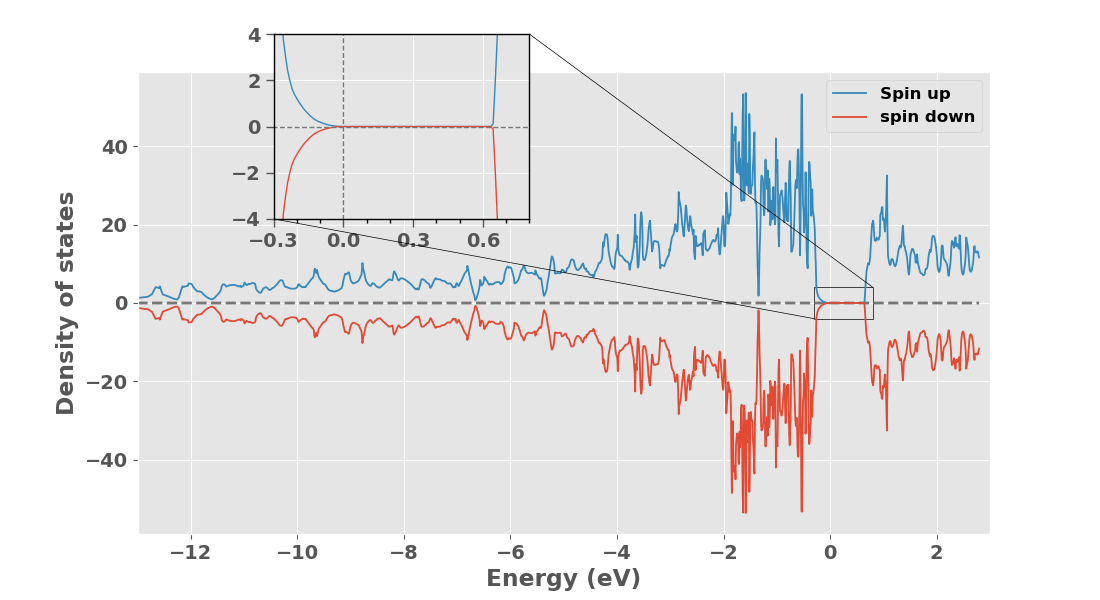
\includegraphics[width=\textwidth]{results/fesi2/bulk_DOS.png}
\caption{Density of states (PBE) $\beta-$ \ch{FeSi2}}
\end{figure}
 

\section{\ch{(CrFeMnNi)Si2} SQSs}
Below in table 7.1 we list the total energy per atom (Toten), final magnetic moment per atom (Mag) and band gap ($E_G$) of five unique SQSs of the \ch{Cr4Fe4Mn4Ni4Si32} alloys based on the $\beta-$ \ch{FeSi2} structure. In addition we include the mean and standard deviation (std) between the 5 supercells and the formation energy calculated from the mean total energy. Details on the generation and general features of the alloys is provided in section 6.2. 
 
\begin{table}[H]
\centering
\begin{tabular}{@{}cccc@{}}
\toprule
SQS           & \begin{tabular}[c]{@{}c@{}}Toten \\ (eV)\end{tabular} & \begin{tabular}[c]{@{}c@{}}Mag \\ ($\mu_B$)\end{tabular} & \begin{tabular}[c]{@{}c@{}}$E_G$ \\ (eV)\end{tabular} \\ \midrule
A             & -6,6080                                               & 0.0833                                                   & 0.0280                                                \\
B             & -6,6138                                               & 0.0833                                                   & 0.0523                                                \\
C             & -6,6063                                               & 0.0834                                                   & 0.0344                                                \\
D             & -6,6155                                               & 0.0833                                                   & 0                                                     \\
E             & -6,6089                                               & 0.0833                                                   & 0.0495                                                \\ \midrule
Mean          & -6.6105                                               & 0.0833                                                   & 0.0328                                                \\
Std           & 0.0039                                                & 0.0000                                                   & 0.0210                                                \\
$E_{FPA} (eV)$   & -0.293                                          & -                                                        & -                                                     \\ \bottomrule
\end{tabular}
\caption{Total energy per atom, final magnetic moment and band gap of 5 unique SQS of \ch{(CrFeMnNi)Si2} based on the $\beta-$ \ch{FeSi2} unit cell.}
\end{table}

From table 7.1 we observe that the total energy and magnetic moment are quite similar in all 5 supercells, which could be expected from that the atomic configuration is the only variable. On the other hand the atomic configuration have a larger impact on the band gap of the supercells. We find that the band gap ranges from a maximum value of 0.05 eV in SQS B, to a metal in SQS D, nevertheless much smaller than \ch{FeSi2} (0.65 eV). We will come back to discussing the band gaps in later sections. 

Compared to the bulk material we find that the alloy apparent from all five supercells display a finite magnetic moment of around $0.083 \mu_B$. The local magnetic moments show some variation between supercells but follow the same trend where the largest moments are attributed to chromium atoms in the lattice, followed by manganese. On the other side the magnetic moments of both iron and nickel within the numerical accuracy of the calculations give negligible contributions to the magnetic moment of the structures. Considering that the total magnetic moment is identical in 5 distinct atomic configurations and the local magnetic moments show very similar trends, the observed magnetism within the scope of this project is most probably connected to the particular crystal structure. It should be noted however that the magnetic properties in this project could be prone to errors. As we discussed in section 4.3 one of the major drawbacks of DFT in regards to magnetic materials is the local minima problem. In this project we have overlooked this concern and applied a constant initial co-linear magnetic configuration in all structures in order to reduce the workload, thus it's possible that the final magnetic structure of the supercells adopt local minimas rather than global. Coupling this with the possible errors associated with the special quasi-random structures method to model the disordered magnetic structure means that the magnetic results and following the total energy and corresponding stability are not immutable nor necessarily accurate in respect to the hypothetical real alloy. 
    
In terms of the total energy the most and least stable SQSs are "D" and "A" respectively, meaning that SQS D is then the most representative configuration of the real material. However most likely all five SQSs and other possible configurations would appear as local orderings in domains of the real material with a certain probability. Therefore we will consider and discuss the results of all 5 SQSs as well as the most stable supercell. Further the total energy alone is not sufficient to evaluate the stability of the structure. In this project we have not considered factors such as the configurational entropy or made any finite temperature considerations in general. Additionally the discussion above on the magnetic configuration could affect the total energy. Thus the relative stability between supercells listed in table 7.1 could be  variable, nevertheless the most stable configuration is moderately emphasized from the considerations made in this project.
 
\newpage
\subsection{The band gap}
As seen from table 7.1 the band gap of the alloy are severely reduced from the bulk material, and vary from supercell to supercell. We observed a maximum band gap of 0.05 eV in SQS B, and on the flip side a 0 band gap in the utmost stable configuration SQS D. The density of states of SQS D and B is displayed in figures 7.2 and 7.3 below, similar plots can be found in appendix [REF] for the other supercells. 

\begin{figure}[H]
	\centering
	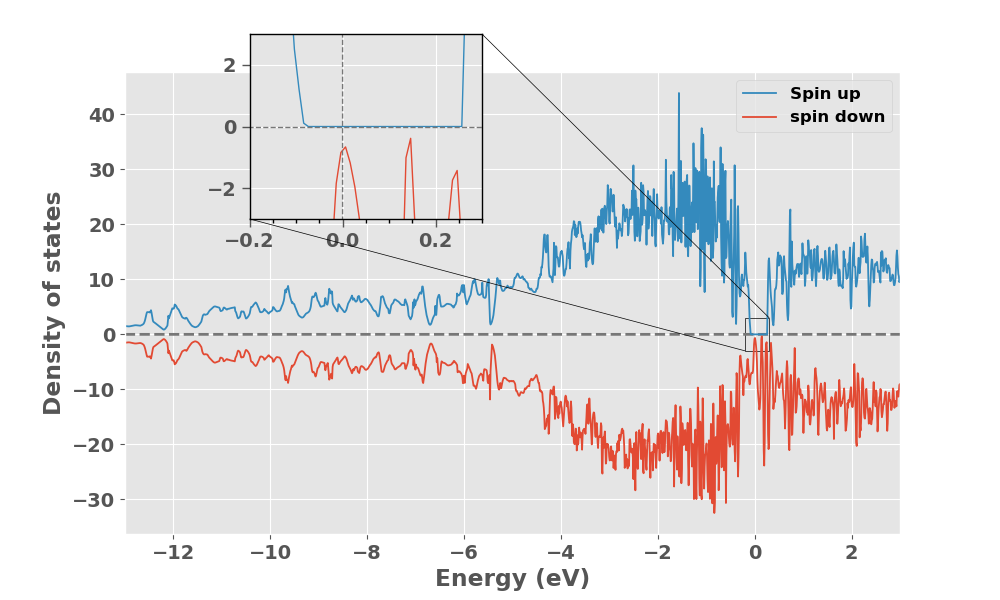
\includegraphics[width=\textwidth]{results/fesi2/D_TDOS.png}
	\caption{Density of states of SQS D \ch{(CrFeMnNi)Si2} with PBE.}
\end{figure}

\begin{figure}[H]
\centering
	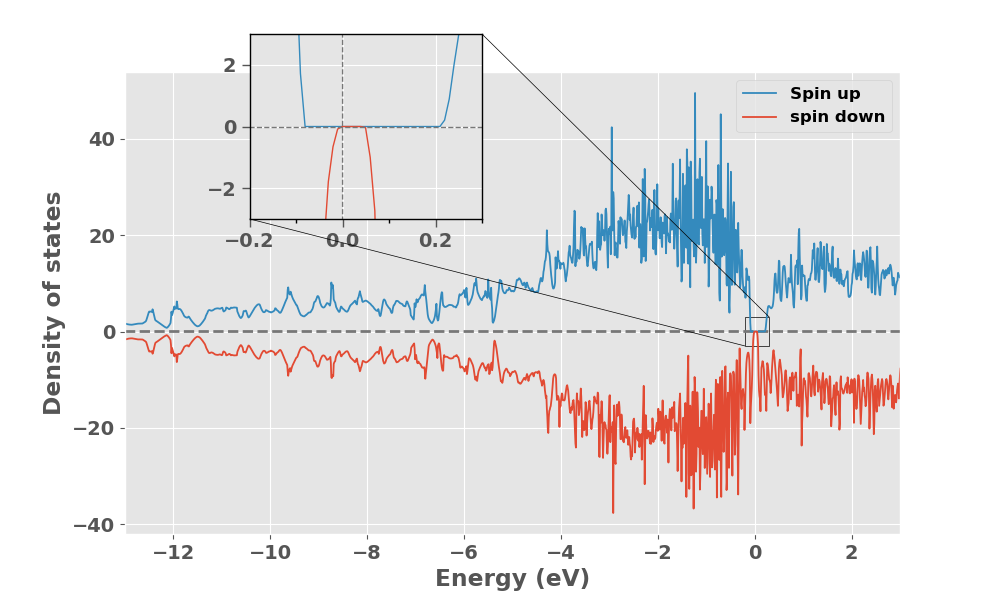
\includegraphics[width=\textwidth]{results/fesi2/B_TDOS.png}
	\caption{Density of states of SQS B \ch{(CrFeMnNi)Si2} with PBE.}
\end{figure}  

In figure 7.2  and 7.3 we observe that the band gap in both SQS D and B in accordance with the magnetic property is different between spins. Going forward we will refer to the band gap in spin up as $E_G ^\text{up}$, and spin down as $E_G ^\text{dw}$. Clearly in both D and B $E_G ^\text{up} >> E_G ^\text{dw}$ as SQS D for instance exhibits a band gap of around 0.3 eV in spin up, contrary to a 0 band gap in spin down. Comparing to the values in table 7.1 we find that the total band gaps of the respective structures is limited by the narrow or nonexistent band gap in spin down. To obtain further and more precise information on the band gap we look to the calculated Kohn-Sham eigenvalues. The eigenvalue band gaps, denoted as $E_G ^\text{eigen}$ can be seen below in table 7.2 for all five SQS, where the utmost stable configuration (SQS D) is highlighted in bold text. Continuing the trend described above we observe equivalent to SQS D and B that $E_G ^\text{up} >> E_G ^\text{dw}$ for all supercells, par SQS A where the spin polarization of the band gap is less prominent and the total band gap is the combined sum of $E_G ^\text{up}$ and $E_G ^\text{dw}$.

\begin{table}[H]
\centering
\begin{tabular}{@{}cccc@{}}
\toprule
SQS & \begin{tabular}[c]{@{}c@{}}$E_G ^\text{up, eigen}$ \\ (meV)\end{tabular} & \begin{tabular}[c]{@{}c@{}}$E_G ^\text{dw, eigen}$ \\ (meV)\end{tabular} & \begin{tabular}[c]{@{}c@{}}$E_G ^\text{tot, eigen}$ \\ (meV)\end{tabular} \\ \midrule
A   & 81.4                                                                     & 52.2                                                                     & 28.1                                                                    \\
B   & 293                                                                      & 52.2                                                                     & 52.2                                                                    \\
C   & 236                                                                      & 34.3                                                                     & 34.3                                                                    \\
\textbf{D}   & 339                                                                      & 0.00                                                                     & 0.00                                                                    \\
E   & 308                                                                      & 50.0                                                                     & 50.0                                                                    \\ \bottomrule
\end{tabular}
\caption{Band gap of the 5 SQSs of \ch{(CrFeMnNi)Si2} calculated from the eigenvalues in spin up, down and total.}
\end{table}

In VASP the energy eigenvalues are listed for every energy band at all k-points used in the calculation, with corresponding occupancy. An occupancy of 1 represents a fully occupied eigenstate, in analog a completely unoccupied (empty) eigenstate have occupancy equal to 0. Recalling that occupied states belong to the valence band, and the conduction band consists of unoccupied states (at 0 K). The highest energy valence band in these structures are band 124 in spin down and 128 in spin up, following the lowest energy valence band is 125/129 in spin down/up. The band gap in spin down is then determined from the difference between the lowest energy eigenvalue in band 125 and the highest energy eigenvalue in band 124, and likewise for the spin up band gap between bands 128 and 129. In SQS D different from the semiconducting structures we observe some partially occupied states at the band edges in bands 124 and 125 in spin down. With partially occupied states we refer to eigenstates in the valence band with occupancy less than 1 and states in the conduction band with occupancy above 0. Specifically the highest energy eigenvalue (9.01 eV) in band 124 have occupancy equal to 0.94, and equivalently the lowest energy eigenvalue (8.98 eV) in band 125 have occupancy equal to 0.08. This results in a 0 (negative) band gap. Further the Fermi energy in this structure is 8.99 eV, the partially occupied eigenstate in band 124 is then above the Fermi energy, and the partially unoccupied eigenstate in the conduction band below the Fermi energy. This is a clear indication of a metal, in which the conduction band and valence band overlap. In this project we will refer to such eigenstates with partial occupancy as defect states. The importance of the defect states on the band gap in SQS D can be seen clearly in table 7.3. Here we calculate the band gap as a function of the defect states by an occupancy parameter $occ$, such that $E_G (0.99, 0.01)$ is the band gap when only including eigenvalues with corresponding occupancy above 0.99 in the valence band and below 0.01 in the conduction band. For simplicity we will write the parameter as a single value, where $occ = 0.01$ represents occupancy equal to 1 - 0.01 in the valence band and 0 + 0.01 in the conduction band.

\begin{table}[H]
\centering
\begin{tabular}{@{}cccc@{}}
\toprule
occ              & \begin{tabular}[c]{@{}c@{}}$E_G ^\text{up, eigen}$ \\ (meV)\end{tabular} & \begin{tabular}[c]{@{}c@{}}$E_G ^\text{dw, eigen}$ \\ (meV)\end{tabular} & \begin{tabular}[c]{@{}c@{}}$E_G ^\text{tot, eigen}$ \\ (meV)\end{tabular} \\ \midrule
0.5              & 339                                                                      & 0                                                                        & 0                                                                       \\
0.05             & 339                                                                      & 21.0                                                                     & 21.0                                                                    \\
0.01             & 339                                                                      & 49.6                                                                     & 49.6                                                                    \\
0.001            & 339                                                                      & 73.3                                                                     & 73.3                                                                    \\
\textless 0.0001 & 339                                                                      & 85.7                                                                     & 85.7                                                                    \\ \bottomrule
\end{tabular}
\caption{Band gap of SQS D as a function of occupancy in the eigenvalues.}
\end{table}

From table 7.3 we find clear evidence of the defect states prohibiting the band gap in spin down in SQS D, compared to the semiconducting supercells that contain only fully occupied and unoccupied eigenstates. To investigate this effect to greater extent we compare the eigenvalues of SQS D to a pure metal, such as iron. In this case the energy bands (both spins) around the Fermi energy (5.8 eV) is populated mostly by partially filled eigenstates. Inside a single energy band we observe instances of both more than half-filled states above $E_F$, and less than half-filled states above $E_F$, thus clearly overlap between the conduction and valence band. In contrast we find no instances of partial occupants in pure Si, as in the semiconducting SQSs. Therefore we can firmly state that the "defect states" are associated with a metallic character. Compared to the pure metal however, the amount and severity of the partial occupants are very dampened in SQS D. The concept of defect or impurity states in the band gap have been found as a common feature of the band structure of random alloys \cite{PhysRevLett.104.236403}, however we have reservations about if this is a physical result or related to numerical factors. In addition to partial occupants in Fe and SQS D we observe a plural of non-naturalistic states where the occupancy exceeds 1 and 0. Recalling that the discontinues Fermi surface of metals poses several obstacles on DFT calculations with respect to the smearing and number of k-points. This result could then be imagined as a consequence of numerical methods. For instance in SQS B we conducted three separate electronic calculations, one with the tetrahedron method (value listed in tables) and two calculations with Gaussian smearing with smearing width 0.05 and 0.005 eV. With the Gaussian method and smearing width $\sigma = 0.05 eV$ we get $E_G ^\text{up, eigen} = 0.2987 eV$ and $E_G ^\text{dw, eigen} = 0.0497 eV$. Further calculations with the Gaussian method with smearing width of 0.005 eV results in $E_G ^\text{up, eigen} = 0.2932 eV$ and $E_G ^\text{dw, eigen} 0.0522 eV$. Compared to the values in table 7.3 with TBC, we observe that Gaussian (0.005 eV) and TBC are identical, while Gaussian (0.05 eV) show some deviation. Furthermore we find that the eigenvalues of Gaussian 0.05 eV contain defect states, and that the spin down band gap can thus be enlarged as in SQS D previously by $E_G ^\text{dw, eigen}(0.01) = 0.1695 eV$. However, in this case we find no instances of non-naturalistic states as we described above for SQS D with TBC.
  
In conclusion, the defect states observed in SQS D is clearly related to metallic properties, however from the discussion above we have seen that the results could be subjected to numerical factors as well. It would have been instructive to visualize and analyze the eigenvalues by plotting the band structure. Unfortunately this is neither simple to perform or interpret in large supercells consisting of several elements and a large number of energy bands. One solution to this is to perform band-unfolding, but this did not work in conjunction with the TDEP implementation of the special quasi-random structures method. 


\newpage
\subsection{Local and projected density of states}
In this section we will analyze the local and projected density of states of primarily SQS D (most stable). Below we include the local density of states of silicon in figure 7.4, and the respective LDOS plots of the various 3d elements of the compound in figure 7.5.  
  
\begin{figure}[H]
	\centering
	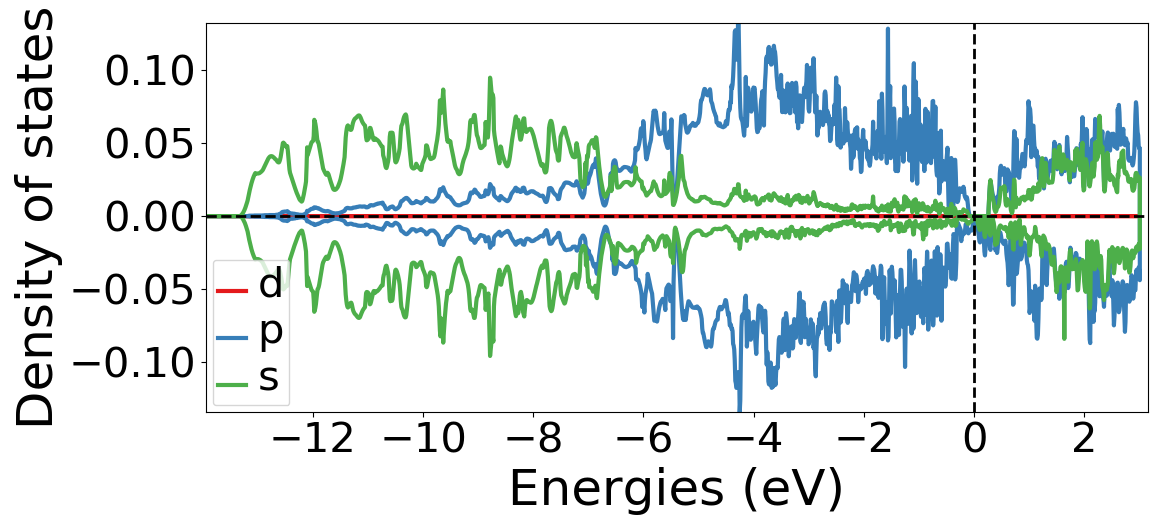
\includegraphics[width=.7\textwidth]{results/fesi2/D_LDOS_Si.png}
	\caption{Local density of states of Si (SQS D)}
\end{figure} 

\begin{figure}[H]
	\centering
	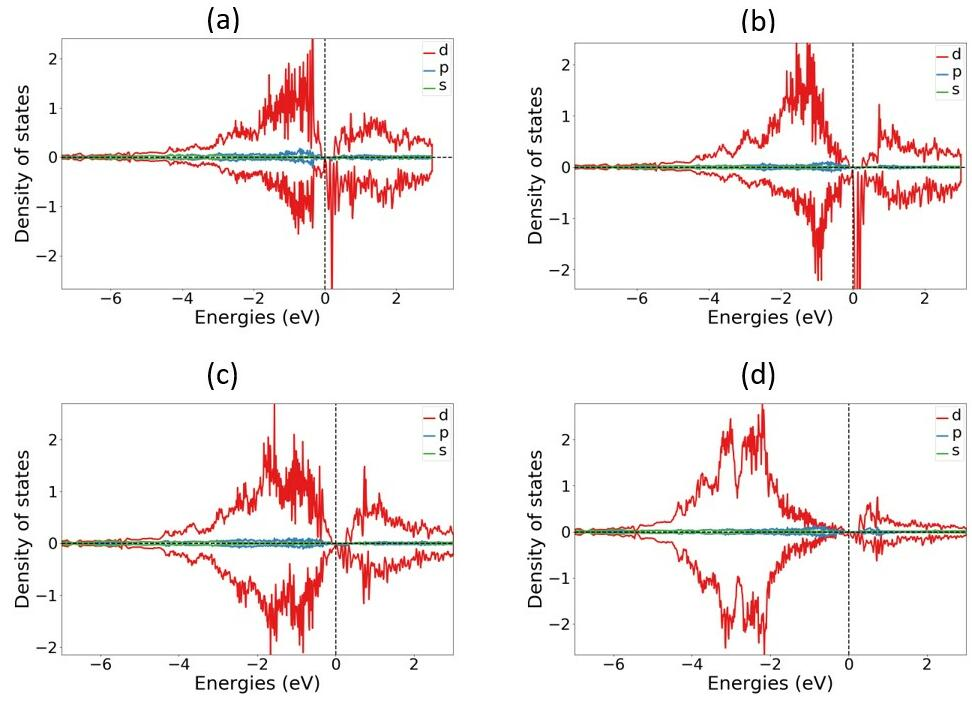
\includegraphics[width=\textwidth]{results/fesi2/D_LDOS.jpeg}
	\caption{Local density of states of (a) Cr, (b) Mn, (c) Fe, (d) Ni in SQS D.}
\end{figure}   
  
In the local density of states plotted in figure 7.4 we see that the s-electrons in Si occupy states in the lower energy regions and p electrons at slightly elevated energies closer to the Fermi energy. Above $E_F$ states are occupied by s and p electrons equally. Between the 3d electrons of the transition metals, markedly manganese and chromium display a strong presence at energies just above $E_F$ and manganese additionally bellow $E_F$. Iron an Nickel show largest contributions at energies further from the Fermi energy, most notably bellow $E_F$. In the spin up channel we see a similar trend where chromium lie closest to $E_F$ followed by manganese, iron and lastly nickel at the lowest energies. It could also be noted that in relation to the local magnetic moments discussed previously, we observe that the local density of states is symmetric with respect to spin in Fe and Ni, but not in Cr and Mn. 

\begin{figure}[H]
	\centering
	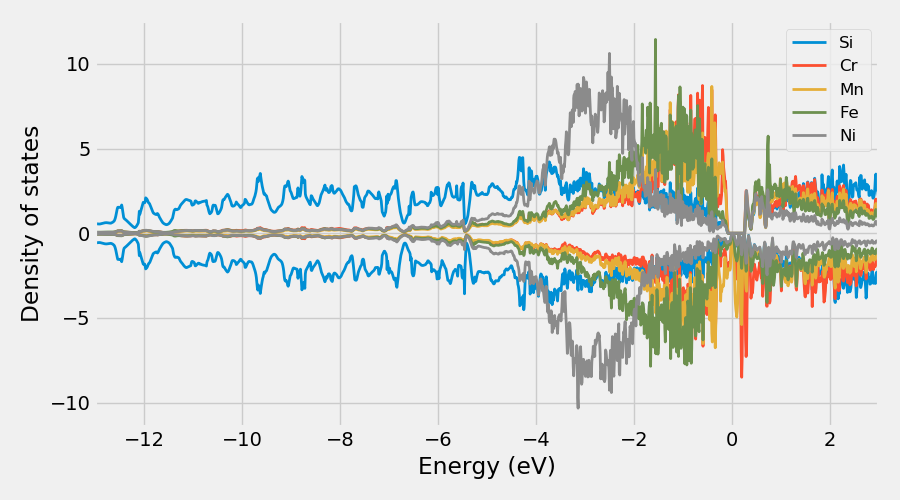
\includegraphics[width=.8\textwidth]{results/fesi2/D_PDOS.png}
	\caption{Projected density of states SQS D CFMN (fesi2) from PBE calculation}
\end{figure} 

The interplay between 3d elements and silicon as shown in the projected density of states (figure 7.6) is in good agreement with observed trends in simpler Si-rich transition metal silicides \cite{lange1997electronic} and Fe and Si $\beta-$ \ch{FeSi2} \cite{doi:10.1063/1.346415}.
\begin{figure}[H]
	\begin{subfigure}{.5\textwidth}
			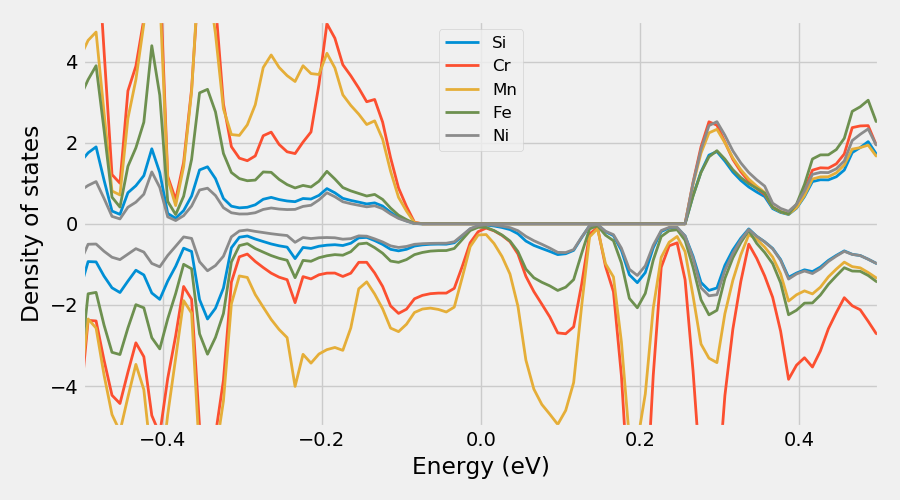
\includegraphics[width=\textwidth]{results/fesi2/D_PDOS_Ef.png}
			\caption{SQS D}		
	\end{subfigure}
	\begin{subfigure}{.5\textwidth}
		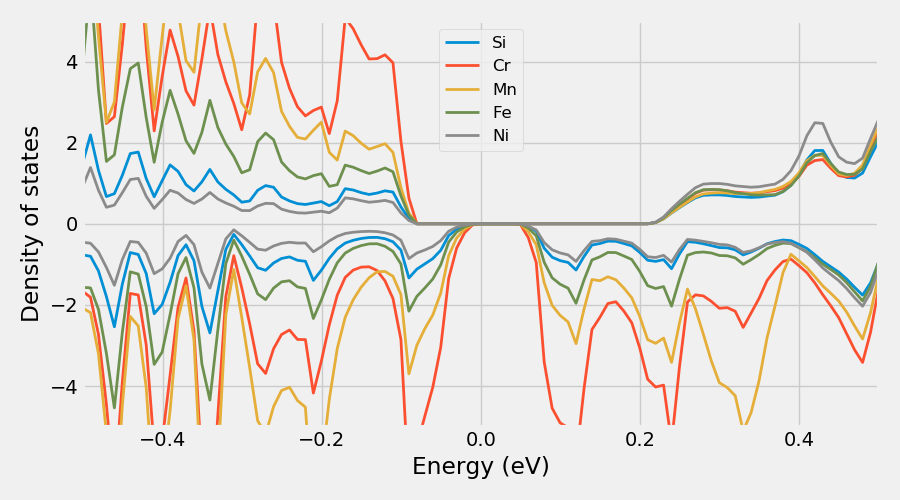
\includegraphics[width=\textwidth]{results/fesi2/B_PDOS_Ef.png}
		\caption{SQS B}		
	\end{subfigure}
	\caption{Projected density of states of SQS D and B around $E_F$}
\end{figure}

Comparing the PDOS of half-metallic SQS D (figure 7.7 a) to the configuration with the largest $E_G ^\text{dw}$) SQS B (figure 7.7 b), we find distinctly a large number of Mn states in SQS D around $E_F$ most noticeably in spin down, but also in spin up. The PDOSs of the other 3 SQSs is included in appendix .. 

\subsection{The band gap with SCAN and HSE06}
As expressed previously, in this work we invoke 3 level of depths GGA (PBE), meta-GGA (SCAN) and hybrid functional (HSE06) to determine the band gap. The outcome of these 3 functionals are showcased in table 7.4.

\begin{table}[H]
\centering
\begin{tabular}{@{}ccccc@{}}
\toprule
\multicolumn{1}{l}{SQS}                 & XC-functional & \begin{tabular}[c]{@{}c@{}}$E_G ^\text{up}$ \\ (eV)\end{tabular} & \begin{tabular}[c]{@{}c@{}}$E_G ^\text{dw}$ \\ (eV)\end{tabular} & \begin{tabular}[c]{@{}c@{}}$E_G ^\text{tot}$ \\ (eV)\end{tabular} \\ \midrule
\multicolumn{1}{c|}{\multirow{3}{*}{A}} & PBE           & 0.0815                                                           & 0.0521                                                           & 0.0281                                                            \\
\multicolumn{1}{c|}{}                   & SCAN          & 0                                                                & 0                                                                & 0                                                                 \\
\multicolumn{1}{c|}{}                   & HSE06         & 0.7084                                                           & 0.0261                                                           & 0.0261                                                            \\ \midrule
\multicolumn{1}{c|}{\multirow{3}{*}{B}} & PBE           & 0.2932                                                           & 0.0523                                                           & 0.0523                                                            \\
\multicolumn{1}{c|}{}                   & SCAN          & 0.1470                                                           & 0.0890                                                           & 0.0890                                                            \\
\multicolumn{1}{c|}{}                   & HSE06         & 0.2855                                                           & 0.1819                                                           & 0.1819                                                            \\ \midrule
\multicolumn{1}{c|}{\multirow{3}{*}{C}} & PBE           & 0.2355                                                           & 0.0343                                                           & 0.0343                                                            \\
\multicolumn{1}{c|}{}                   & SCAN          & 0.0690                                                           & 0.1124                                                           & 0.1124                                                            \\
\multicolumn{1}{c|}{}                   & HSE06         & 0.1744                                                           & 0.0328                                                           & 0.0196                                                            \\ \midrule
\multicolumn{1}{c|}{\multirow{3}{*}{D}} & PBE           & 0.3386                                                           & 0                                                                & 0                                                                 \\
\multicolumn{1}{c|}{}                   & SCAN          & 0                                                                & 0.1086                                                           & 0                                                                 \\
\multicolumn{1}{c|}{}                   & HSE06         & 0.3780                                                           & 0                                                                & 0                                                                 \\ \midrule
\multicolumn{1}{c|}{\multirow{3}{*}{E}} & PBE           & 0.3078                                                           & 0.0495                                                           & 0.0495                                                            \\
\multicolumn{1}{c|}{}                   & SCAN          & 0.1540                                                           & 0.1112                                                           & 0.1048                                                            \\
\multicolumn{1}{c|}{}                   & HSE06         & 0.5476                                                           & 0.0133                                                           & 0.0133                                                            \\ \bottomrule
\end{tabular}
\caption{Band gap calculated with PBE, SCAN and HSE06 XC-functionals of \ch{(CrFeMnNi)Si2} SQSs.}
\end{table}


We will begin dissecting table 7.4 by comparing SCAN to PBE. The first distinction we make notice of is in SQS A. In this supercell calculations with the SCAN functional predicts a metallic compound, contrary to the the PBE band gap of 0.03 eV. Alike the band gap of SQS D discussed previously, the 0 band gap in this structure with SCAN is caused by defect states. Neglecting such states and evaluating the band gap from just completely filled and empty eigenstates yield $E_\text{G, SCAN} ^{up, eigen}(0.99, 0.01) = 0.0316$ eV and $E_\text{G, SCAN} ^{dw, eigen}(0.99, 0.01) = 0.0531$ eV, and a total band gap of 0.0316 eV. This value seems to agree better with the PBE band gap of this supercell, but we observe that $E_G ^\text{up}$ is larger in PBE.  This is a recurrent patter with SCAN across all five SQSs, where $E_\text{G, SCAN} ^\text{up} < E_\text{G, PBE} ^\text{up}$, and moreover $E_\text{G, SCAN} ^\text{dw} > E_\text{G, PBE} ^\text{dw}$. This can be seen in figure 7.8, where we plot the density of states of SQS E (a, b) and C (c, d). Note that the SCAN band gap in SQS C have the opposite spin polarization of PBE, this is also the case in SQS D as seen from table 7.4.
\begin{figure}[H]
	\begin{subfigure}{.5\textwidth}
		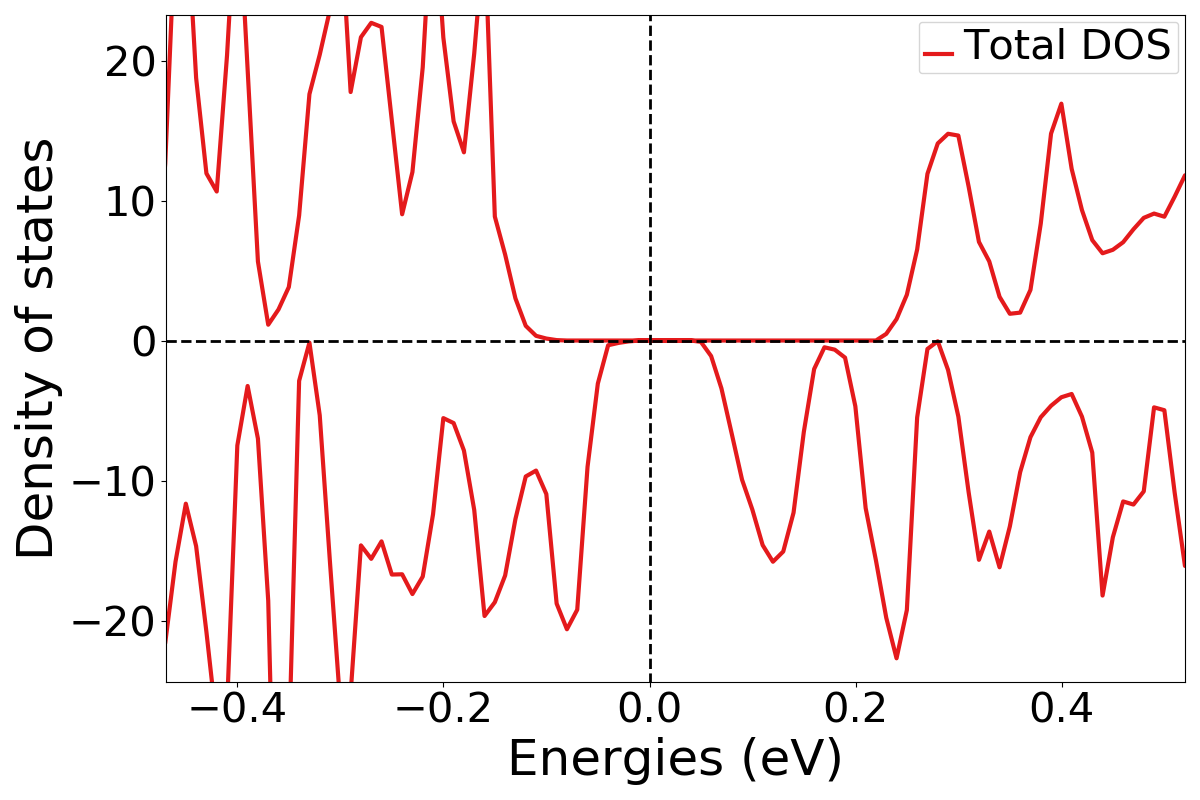
\includegraphics[width=\textwidth]{results/fesi2/E_DOS_pbe.png}
		\caption{SQS E PBE}
	\end{subfigure}
	\begin{subfigure}{.5\textwidth}
		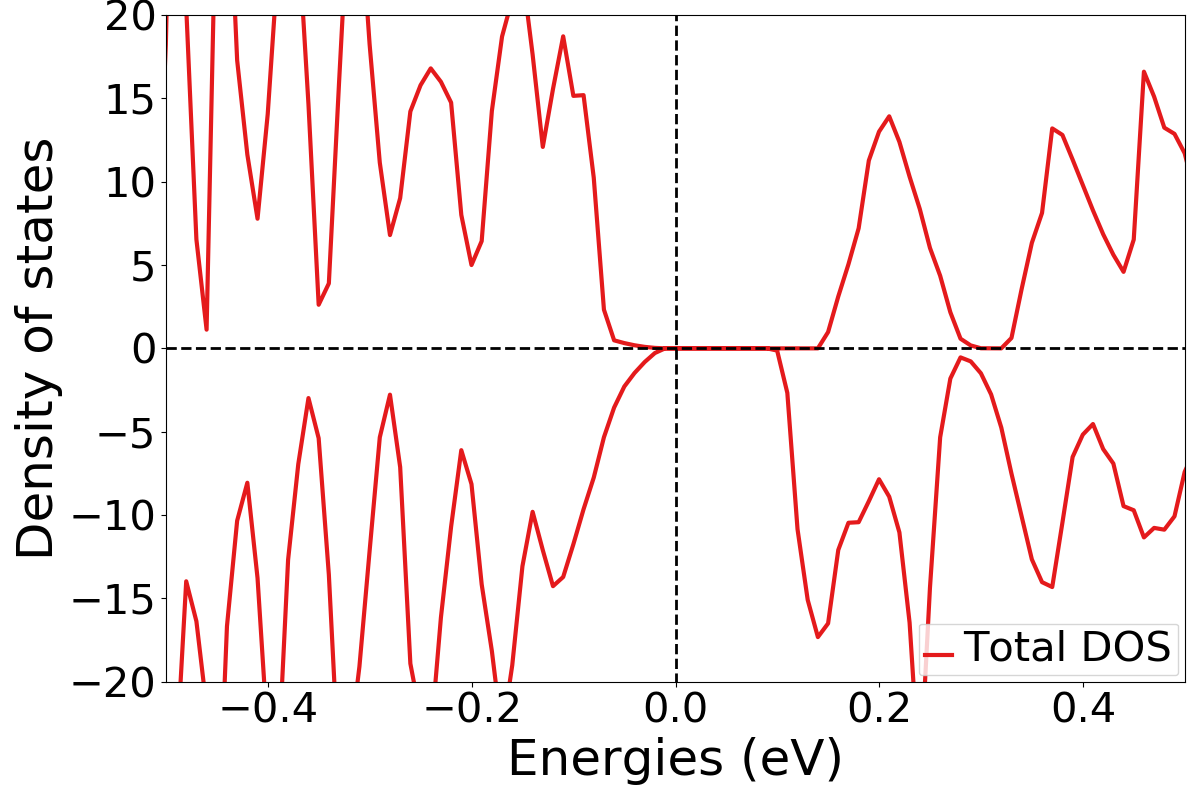
\includegraphics[width=\textwidth]{results/fesi2/E_DOS_scan.png}
		\caption{SQS E SCAN}
	\end{subfigure}
	\begin{subfigure}{.5\textwidth}
		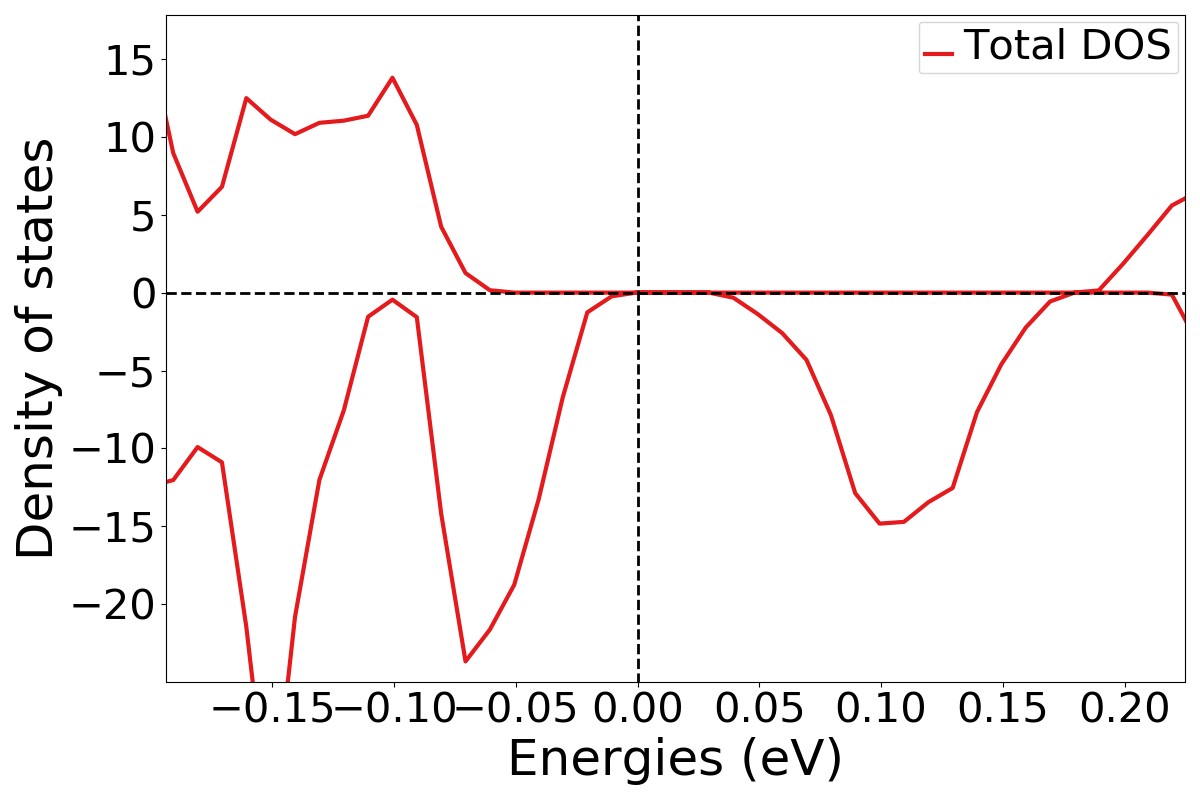
\includegraphics[width=\textwidth]{results/fesi2/C_DOS_pbe.png}
		\caption{SQS C PBE}
	\end{subfigure}
	\begin{subfigure}{.5\textwidth}
		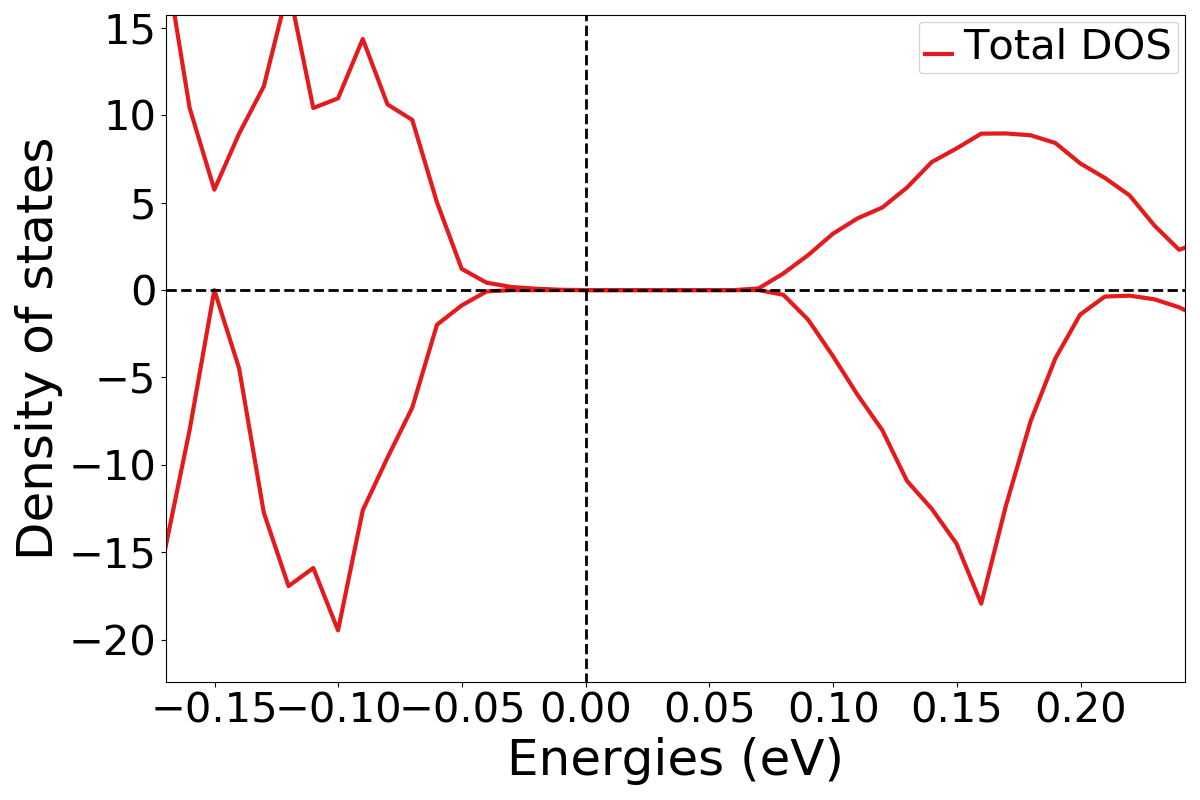
\includegraphics[width=\textwidth]{results/fesi2/C_DOS_scan.png}
		\caption{SQS C SCAN}
	\end{subfigure}
	\caption{Density of states illustrating the band gaps from PBE and SCAN calculations for SQS E and D.}
\end{figure}

With the HSE06 functional we observe the opposite trend to SCAN in SQS A and E, where $E_\text{G, HSE06} ^\text{up} > E_\text{G, PBE} ^\text{up}$ and $E_\text{G, HSE06} ^\text{dw} < E_\text{G, PBE} ^\text{dw}$. But in other cases $E_\text{G, HSE06} ^\text{up}$ is lesser (SQS C) or similar to PBE (SQS B and D). On the other hand $E_\text{G, HSE06} ^\text{dw}$ is consistently smaller in all structures compared to PBE, with the exception of SQS B. In this structure the HSE06 functional predicts large band gaps in both spins, as seen from the density of states plotted in figure 7.8.    
 
 
\begin{figure}[H]
	\centering	
	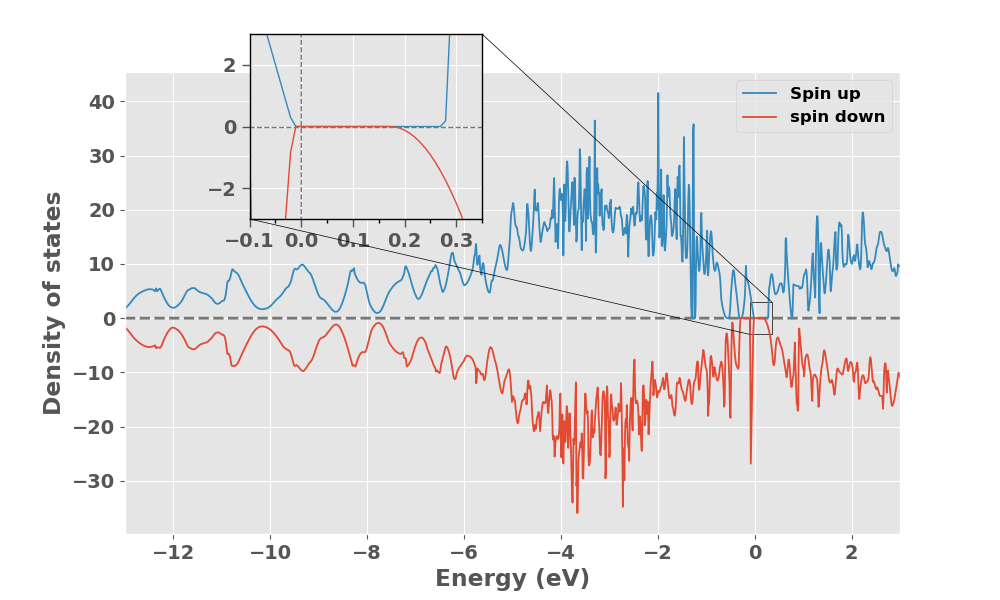
\includegraphics[width=.85\textwidth]{results/fesi2/B_TDOS_hse06.png}
	\caption{Density of states of SQS B with HSE06}
\end{figure}
  
As we discussed in section 5.1, hybrid functionals are much more computationally demanding compared to both meta-GGA and GGA functionals. In this project we experienced particular difficulty of converging calculations with HSE06 of the compositionally complex structures. To reduce the cost of the HSE06 functional we performed such calculations with a lower density of k-points, see section 6.1. The small amount of k-points could as discussed lead to numerical inaccuracies relating to the calculation of the Fermi surface in metallic structures. Furthermore the reduced mesh of k-points could result in artificially exaggerated band gaps from failing to encapsulate the exact minimum transition between the valence band and conduction band.

\begin{table}[H]
\centering
\begin{tabular}{@{}lc@{}}
\toprule
XC-functional & \begin{tabular}[c]{@{}c@{}}Transition \\ (k-point)\end{tabular} \\ \midrule
PBE           & (0.250,0.000,0.250) $\rightarrow$ (0.000,0.000,0.000)           \\
SCAN          & (0.250,0.000,0.250) $\rightarrow$ (0.000,0.333,0.000)           \\
HSE06         & (0.500,0.000,0.000) $\rightarrow$ (0.000,0.000,0.000)           \\ \bottomrule
\end{tabular}
\caption{Minimum gap between k-point in valence band and conduction band in SQS B from PBE, SCAN and HSE06}
\end{table}

In table 7.5 we list the transition between the highest occupied k-state in the valence band and lowest unoccupied k-state in the conduction band for SQS B with PBE, SCAN and HSE06 respectively. We  
observe that all 3 functionals find different band gaps. A concerning factor is that the highest energy k-point in the valence band from PBE calculations (0.250, 0.000, 0.250) is not included in the HSE06 calculation with the narrow mesh of 2x2x2 k-points. Thus one may suspect that the HSE06 calculation overlook the minimum transition and hence return a enlarged band gap instead. This could be the case in $E_\text{G, A} ^{up}$ and $E_\text{G, B} ^{dw}$ where HSE06 predicts much larger values to PBE. However without an experimental baseline we can not conclude that this is the case. As in the other instances we find that HSE06 produce similar or lower band gaps compare to PBE despite of the smaller number of k-points.     

As stated in section 6.2, we did not manage to converge hybrid calculations with the tetrahedron method, and overcame this problem by first calculating the charge density with Gaussian smearing and utilize the density to expedite TBC HSE06 calculations. The respective band gaps from these methods are displayed in table 7.6 for the five SQSs of the \ch{(CrFeMnNi)Si2} system. Here we calculate the band gap from the eigenvalues at different cutoff occupancy $occ$ to highlight the part of defect states. Gaussian smearing was tested with smearing width $sigma$ equal to 0.05 eV and 0.005 eV.

\newpage
\begin{landscape}
\begin{table}[]
\vskip-1.5cm \hskip1cm \begin{tabular}{@{}cccccccc@{}}
\toprule
\multicolumn{1}{l}{SQS}                          & \begin{tabular}[c]{@{}c@{}}Smearing (type) \\ width (eV) \end{tabular} & \begin{tabular}[c]{@{}c@{}}$E_\text{G} ^{up, eigen}(0.5)$\\ (eV)\end{tabular} & \begin{tabular}[c]{@{}c@{}}$E_\text{G} ^{dw, eigen}(0.5)$\\ (eV)\end{tabular} & \begin{tabular}[c]{@{}c@{}}$E_\text{G} ^{up, eigen}(0.99)$\\ (eV)\end{tabular} & \begin{tabular}[c]{@{}c@{}}$E_\text{G} ^{dw, eigen}(0.01)$\\ (eV)\end{tabular} & \begin{tabular}[c]{@{}c@{}}$E_\text{G} ^{tot, eigen}(0.5)$\\ (eV)\end{tabular} & \begin{tabular}[c]{@{}c@{}}$E_\text{G} ^{tot, eigen}(0.99, 0.01)$\\ (eV)\end{tabular} \\ \midrule
\multicolumn{1}{c|}{\multirow{3}{*}{A}}          & \begin{tabular}[c]{@{}c@{}}Gaussian \\ (0.05)\end{tabular}    & 0.7837                                                                        & 0.1493                                                                        & -                                                                              & 0.2984                                                                         & 0.1493                                                                         & 0.2984                                                                                \\
\multicolumn{1}{c|}{}                            & \begin{tabular}[c]{@{}c@{}}Gaussian \\ (0.005)\end{tabular}   & 0.2117                                                                        & 0.1013                                                                        & -                                                                              & -                                                                              & 0.1013                                                                         & -                                                                                     \\
\multicolumn{1}{c|}{}                            & TBC                                                           & 0.7084                                                                        & 0.0261                                                                        & -                                                                              & -                                                                              & 0.0261                                                                         & -                                                                                     \\ \midrule
\multicolumn{1}{c|}{\multirow{3}{*}{B}}          & \begin{tabular}[c]{@{}c@{}}Gaussian \\ (0.05)\end{tabular}    & 0.2783                                                                        & 0.1702                                                                        & 0.2988                                                                         & 0.3136                                                                         & 0.1506                                                                         & 0.2979                                                                                \\
\multicolumn{1}{c|}{}                            & \begin{tabular}[c]{@{}c@{}}Gaussian \\ (0.005)\end{tabular}   & 0.2838                                                                        & 0.1823                                                                        & -                                                                              & -                                                                              & 0.1801                                                                         & -                                                                                     \\
\multicolumn{1}{c|}{}                            & TBC                                                           & 0.2855                                                                        & 0.1819                                                                        & -                                                                              & -                                                                              & 0.1807                                                                         & -                                                                                     \\ \midrule
\multicolumn{1}{c|}{\multirow{3}{*}{C}}          & \begin{tabular}[c]{@{}c@{}}Gaussian \\ (0.05)\end{tabular}    & 0.1078                                                                        & 0.1066                                                                        & 0.2405                                                                         & 0.1839                                                                         & 0.0650                                                                         & 0.1839                                                                                \\
\multicolumn{1}{c|}{}                            & \begin{tabular}[c]{@{}c@{}}Gaussian \\ (0.005)\end{tabular}   & 0.1304                                                                        & 0.0222                                                                        & -                                                                              & -                                                                              & 0.0222                                                                         & -                                                                                     \\
\multicolumn{1}{c|}{}                            & TBC                                                           & 0.1744                                                                        & 0.0328                                                                        & -                                                                              & -                                                                              & 0.0196                                                                         & -                                                                                     \\ \midrule
\multicolumn{1}{c|}{\multirow{3}{*}{\textbf{D}}} & \begin{tabular}[c]{@{}c@{}}Gaussian \\ (0.05)\end{tabular}    & 0.3661                                                                        & 0.0592                                                                        & -                                                                              & 0.1872                                                                         & 0.0592                                                                         & 0.1872                                                                                \\
\multicolumn{1}{c|}{}                            & \begin{tabular}[c]{@{}c@{}}Gaussian \\ (0.005)\end{tabular}   & 0.3736                                                                             & 0.0723                                                                         & -                                                                             & -                                                                             & 0.0723                                                                             & -                                                                                    \\
\multicolumn{1}{c|}{}                            & TBC                                                           & 0.3780                                                                        & 0                                                                             & -                                                                              & 0.2665                                                                         & 0                                                                              & 0.2637                                                                                \\ \midrule
\multicolumn{1}{c|}{\multirow{3}{*}{E}}          & \begin{tabular}[c]{@{}c@{}}Gaussian \\ (0.05)\end{tabular}    & 0.6653                                                                        & 0.1439                                                                        & -                                                                              & 0.1675                                                                         & 0.1439                                                                         & 0.1675                                                                                \\
\multicolumn{1}{c|}{}                            & \begin{tabular}[c]{@{}c@{}}Gaussian \\ (0.005)\end{tabular}   & 0.5825                                                                        & 0.1211                                                                        & -                                                                              & -                                                                              & 0.1211                                                                         & -                                                                                     \\
\multicolumn{1}{c|}{}                            & TBC                                                           & 0.5476                                                                        & 0.0133                                                                        & -                                                                              & -                                                                              & 0.0133                                                                         & -                                                                                     \\ \cmidrule(l){2-8} 
\end{tabular}
\caption{Band gap from HSE06 calculations with Gaussian smearing and smearing width  $sigma$ equal to 0.05 and 0.005, and the tetrahedron method (TBC). "-"  means unchanged}
\end{table}
\end{landscape}
\newpage

From table 7.6 we observe that the presence and affect of defect states as discussed in section 7.2.1 is only present with Gaussian ($\sigma = 0.05 eV$). Alike the previous cases, we find here finite band gaps despite of defect states. By comparing $E_G ^\text{up}$ and $E_G ^\text{dw}$ at $occ = 0.5$ and $occ = 0.01$, the defects appear to have a lesser role in spin up, as par SQS C the band gap in spin up is either consistent or only marginally different between the defect band gap and the hypothetical defect less band gap. $E_G ^\text{dw}$ on the other hand increase significantly by removing the defect states. The Gaussian smearing method is generally in better agreement with TBC at lower smearing width. But even in this case we find several dissimilarities. In A and E $E_G ^\text{dw}$ is larger with the Gaussian method, additionally $E_G ^\text{up}$ is much lower in SQS A. Furthermore the band gap of SQS D with HSE06 is with TBC in good agreement with the half-metallic compound found with PBE, meanwhile the Gaussian method ($\sigma = 0.005 eV$) predicts a semiconductor with band gap equal to $0.07 eV$. In this project we have based our choice of numerical smearing on the advice on the VASP manual that state that for accurate total energies and density of states in semiconductors one should opt for the tetrahedron method \cite{ismear}.  However since our system is comprised of metals as well as Si, we include the results from utilizing Gaussian smearing. There are of course many more factors that affect the accuracy and reliability of both methods, but these are outside the scope of this project.

The fact that all 3 functionals and five SQS in majority agree on the presence of a band gap is in itself an overwhelmingly positive result that allow us to state with high certainty that the potential high-entropy silicide \ch{(CrFeMnNi)Si2} is in fact a semiconductor or possibly a half-metal based on the observed spin polarization and the utmost stable configuration. Regarding the 3 functionals applied in this project, we experience best cohesion between PBE and HSE06 that both agree on a spin up polarization of the band gap, while SCAN predicts more symmetric band gaps. This can also be seen from the magnetic moment, with PBE and HSE06 the final magnetic moment (per atom) is 0.083 $\mu_B$ across all SQSs, with SCAN this is reduced to half the amount. In the nonmagnetic $\beta-$ \ch{FeSi2} structure we find better agreement between PBE and SCAN. Both correctly predict that the material is nonmagnetic, however compared to the experimental value of about 0.85 eV and the PBE band gap of 0.65 eV, we get a smaller band gap of 0.61 eV with SCAN. Thus the SCAN functional does not necessarily result in increased accuracy over PBE even in the nonmagnetic material. To conclude this section on the band gap \ch{(CrFeMnNi)Si2}, when studying the band gap with DFT, particularly PBE is well known to underestimate the band gap of the real material as in \ch{FeSi2}. Therefore a band gap found with PBE would with high probability be replicated/increased in the real material. In the following sections and cases we will heavily emphasize the PBE functional to determine the band gap from both the fast and reliable use in addition to the point mentioned above. Furthermore from our experiences in this project in conjunction with the lack of literary support the SCAN function look to be ill-equipped for accurate band gaps. While the HSE06 functional is often to computationally expensive and troublesome to converge for the structures in this project.
 
\subsection{Pair distribution functions}
The pair distribution functions of SQS D and B can be seen below in figure 7.10, the PDFs corresponding to SQS A, C, and E can be found in appendix .. . We include the PDFs of SQS D and B because as stated D is from the considerations made in this project the most stable atomic configuration and hence the most representative of the real random alloy. We analyze the PDF side by side to SQS B to investigate distinctions between the half-metallic configuration (D) and the semiconducting configuration (B). 
 
\begin{figure}[H]
	\centering
	\begin{subfigure}{\textwidth}
		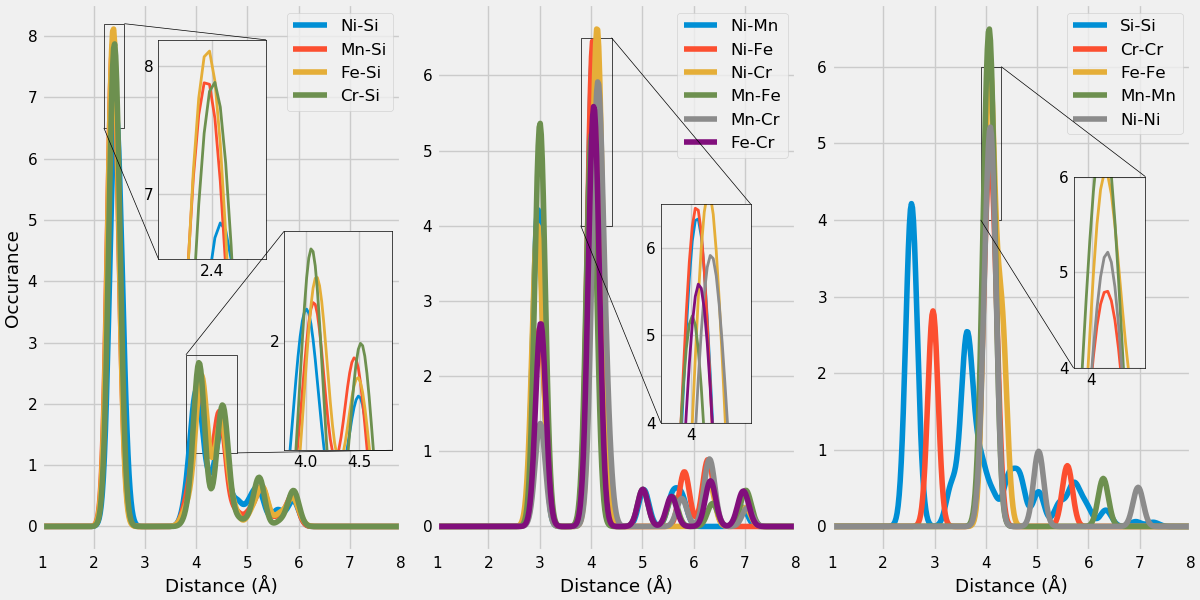
\includegraphics[width=\textwidth]{results/fesi2/D_PDF2.png}
	\end{subfigure}
	\begin{subfigure}{\textwidth}
		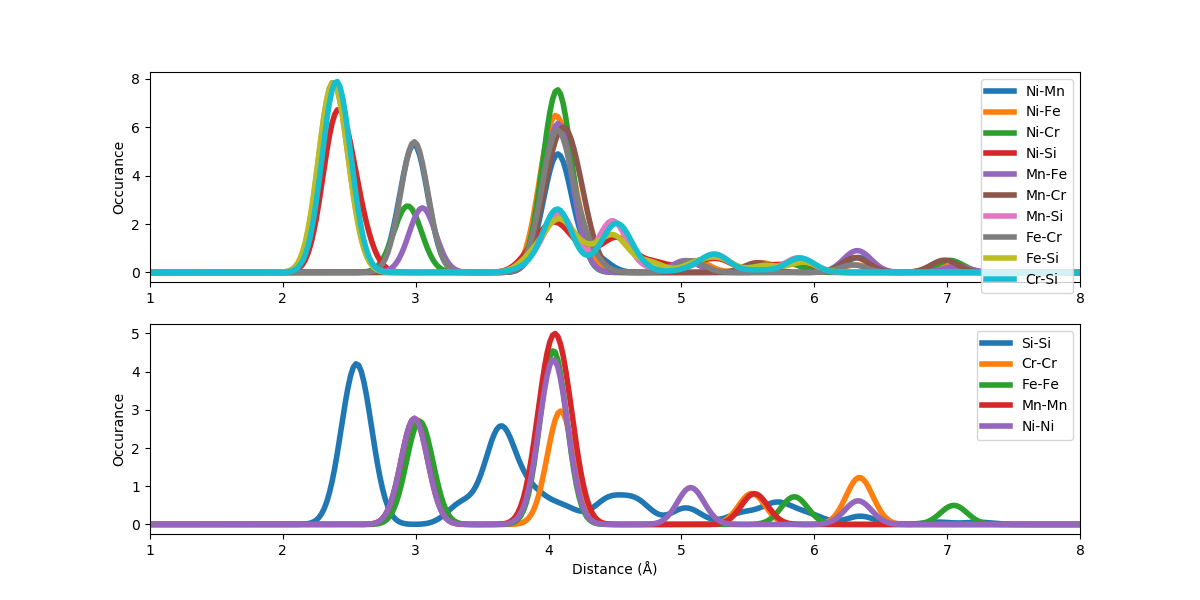
\includegraphics[width=\textwidth]{results/fesi2/B_PDF.png}
	\end{subfigure}
	\caption{Pair distribution functions of SQS D (top) and B (bottom)}
\end{figure}

With the aid of the ICSD \textbf{(insert citation)}, we can compare the PDFs in figure 7.10 to the expected PDFs based on a a large number of experimental compounds. As our compound contain a total of 15 different bonds, comparing each one to the ICSD values would be an exhaustive process. According to the ICSD   the preferred bond-length of TM-Si bonds is observed at two values, with the shorter length the most occurring. Specifically Fe-Si between 2.25-2.75 Å and 4-5 Å, Mn-Si at 2.25-2.75 Å and 3.5-5 Å, Ni-Si between 2.25-2.5 Å and 3.85-5 Å, and finally Cr-Si between 2.35-2.65 Å and 4-5 Å. Clearly, the PDFs of the SQSs are in good agreement with the listed values of TM-Si bonds. The relative occurrence of the bonds between SQS D and B are mostly consistent, other than marginally reduced Fe-Si occurrence at 2.4 Å in B.

In contrast, we observe several distinctions between TM-TM bonds in SQS D and B, for example Mn-Fe, Cr-Fe, and Ni-Mn bonds. This is simply a consequence of how the SQSs are generated, the silicon atoms are placed as before in the new supercells, but the TM elements are "randomly" distributed. Thus, it's reasonable that we would find the major differences between TM-TM bonds. Recalling that Mn had a distinct presence in spin down around $E_F$ in SQS D, we observe that this structure compared to SQS B have a preference of Mn-Fe bonds at 3 Å and show larger occurance of Mn-Mn bonds at 4 Å. However the differences between PDFs are difficult to relate to the observed properties. Firstly because of the shear number of total bonds in the structures, and secondly considering the uniqueness of each SQS paired with the uncertainties regarding the stability.

\newpage
\subsection{SQS size}
Above we have presented the results of a high-entropy silicide \ch{(CrFeMnNi)Si2} investigated by 5 48-atom SQSs with a volume of $700$\r{A}$^3$. This intermediate size allowed us to apply different XC-functionals, and a broad study of different compositions which we will discuss in the next section. However the application of the SQS method to HEAs is not necessarily straightforward as we discussed in section 4.3. The most pressing concern is the size of the SQS model and if it's sufficient enough to correctly model the disordered multi-component structure. In this section we will evaluate this factor by studying the difference between the 48 atom SQSs discussed above to that of 96 and 192-atom SQSs with volume $1200$\r{A}$^3$ and $2400$ \r{A}$^3$ respectively. The computational cost of the 3 sizes are included below in figure 7.11 in terms of the number of CPU hours.

\begin{figure}[H]
\centering
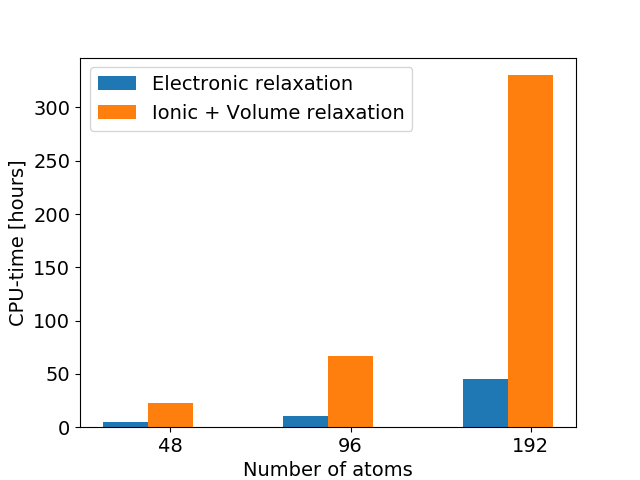
\includegraphics[width=.7\textwidth]{results/SQS_time.png}
\caption{CPU time of 48, 96 and 192-atom SQSs of \ch{(CrFeMnNi)Si2}}
\end{figure}

Alike the 48-atom model, the 96 and 192-atom SQS were tested by 5 unique configurations. In table 7.7 we report the mean and standard deviation from the set of configurations for all three sizes, with respect to the total energy per atom and final magnetic moment per atom, in addition to the formation energy of the mean total energy. 
\begin{table}[H]
\centering
\begin{tabular}{@{}cccccc@{}}
\toprule
SQS size  & \multicolumn{2}{c}{\begin{tabular}[c]{@{}c@{}}Toten\\ (eV)\end{tabular}} & \multicolumn{2}{c}{\begin{tabular}[c]{@{}c@{}}Mag\\ ($\mu_B$)\end{tabular}} & \begin{tabular}[c]{@{}c@{}}$E_{FPA}$\\ (eV)\end{tabular} \\ \midrule
          & mean                                 & std                               & mean                                 & std                                  & mean                                                      \\ \midrule
48 atoms  & - 6.6105                             & ..                                & 0.0833                               & 0.0000                               & -0.292                                                  \\
96 atoms  & - 6.6092                             & 0.0021                            & 0.0708                               & 0.0114                               & -0.292                                                 \\
192 atoms & - 6.6123                             & 0.0022                            & 0.0761                               & 0.0171                               & -0.295                                                 \\ \bottomrule
\end{tabular}
\caption{Total energy, magnetic moment and formation energy of 48, 96 and 192 atom SQSs of \ch{(CrFeMnNi)Si2}}
\end{table}

As seen from table 7.7 the total energy, magnetism  and corresponding formation energy show very minimal variation between all three sizes, thus the 48-atom model is well converged. On the other hand we observe that the larger models contain larger deviation between configurations, this can be expected given the total number of atoms that can vary between configurations. The band gap corresponding to SQSs of each size are listed in table 7.8. First and foremost the band gap is evident in all three and exhibits analogous spin polarization, however the band gap appears to be less frequent and smaller in the larger structures.

\begin{table}[H]
\centering
\begin{tabular}{@{}ccccc@{}}
\toprule
SQS size                                   & SQS        & \begin{tabular}[c]{@{}c@{}}$E_\text{G} ^{up, eigen}(0.5)$ \\ (eV)\end{tabular} & \begin{tabular}[c]{@{}c@{}}$E_\text{G} ^{dw, eigen}(0.5)$ \\ (eV)\end{tabular} & \begin{tabular}[c]{@{}c@{}}$E_\text{G} ^{tot, eigen}(0.5)$\\  (eV)\end{tabular} \\ \midrule
\multicolumn{1}{c|}{\multirow{5}{*}{48 atoms}}  & A          & 0.0815                                                                         & 0.0521                                                                         & 0.0281                                                                          \\
\multicolumn{1}{c|}{}                     & B          & 0.2932                                                                         & 0.0523                                                                         & 0.0523                                                                          \\
\multicolumn{1}{c|}{}                     & C          & 0.2355                                                                         & 0.0343                                                                         & 0.0343                                                                          \\
\multicolumn{1}{c|}{}                     & \textbf{D} & 0.3386                                                                         & 0                                                                              & 0                                                                               \\
\multicolumn{1}{c|}{}                     & E          & 0.3078                                                                         & 0.0495                                                                         & 0.0495                                                                          \\ \midrule
\multicolumn{1}{c|}{\multirow{5}{*}{96 atoms}}  & \textbf{A} & 0.1705                                                                         & 0.0442                                                                         & 0.0367                                                                          \\
\multicolumn{1}{c|}{}                     & B          & 0.1386                                                                         & 0.0270                                                                         & 0.0270                                                                          \\
\multicolumn{1}{c|}{}                     & C          & 0.1347                                                                         & 0.0363                                                                         & 0.0075                                                                          \\
\multicolumn{1}{c|}{}                     & D          & 0.0892                                                                         & 0.0398                                                                         & 0.0398                                                                          \\
\multicolumn{1}{c|}{}                     & E          & 0.1610                                                                         & 0                                                                              & 0                                                                               \\ \midrule
\multicolumn{1}{c|}{\multirow{5}{*}{192 atoms}} & A          & 0.1197                                                                         & 0.0321                                                                         & 0.0321                                                                          \\
\multicolumn{1}{c|}{}                     & B          & 0.1444                                                                         & 0                                                                              & 0                                                                               \\
\multicolumn{1}{c|}{}                     & C          & 0.1867                                                                         & 0                                                                              & 0                                                                               \\
\multicolumn{1}{c|}{}                     & D          & \textit{0.0478}                                                                & \textit{0.0339}                                                                         & 0                                                                               \\
\multicolumn{1}{c|}{}                     & \textbf{E} & \textit{0.0131}                                                                & \textit{0.0184}                                                                         & \textit{0.0131}                                                                          \\ \bottomrule 
\end{tabular}
\caption{Band gap of SQSs of 48, 96 and 192-atoms of \ch{(CrFeMnNi)Si2}. The names are arbitrary, ie A in 48 does not equal A in 96 or A in 192. The values listed in \textit{cursive} indicate a defect band gap.}
\end{table}

Equivalent to structure D in the 48 atom SQS we find that the 0 value in SQS E in the 48 atom model suffers from defect states, and $E_\text{G} ^{dw, eigen}(0.90, 0.10) = 0.016$ eV. The same is true for SQS B and C (192), but require $occ = 0.999, 0.001$ to yield a finite band gap in spin down. The band gap in SQS D and E (192) on the other hand is finite at $occ = 0.5$ but can be enlarged from increasing $occ$, as we described for the Gaussian ($\sigma$ = 0.05 eV) calculations previously. In SQS D (192-atoms) $E_\text{G} ^{up, eigen}(0.99) = 0.075$ eV and $E_\text{G} ^{dw, eigen}(0.01) = 0.05$ eV and similarly $E_\text{G} ^{up, eigen}(0.99) = 0.05$ eV, and $E_\text{G} ^{dw, eigen}(0.01) = 0.048$ eV in SQS E (192-atoms). In such cases where the eigenvalues inclusive of defect states return a finite band gap, the density of states does not. This is seen in figure 7.12 for SQS E in the 192-atom model that clearly have nonzero DOS at $E_F$ in both spins. 

\begin{figure}[H]
\centering
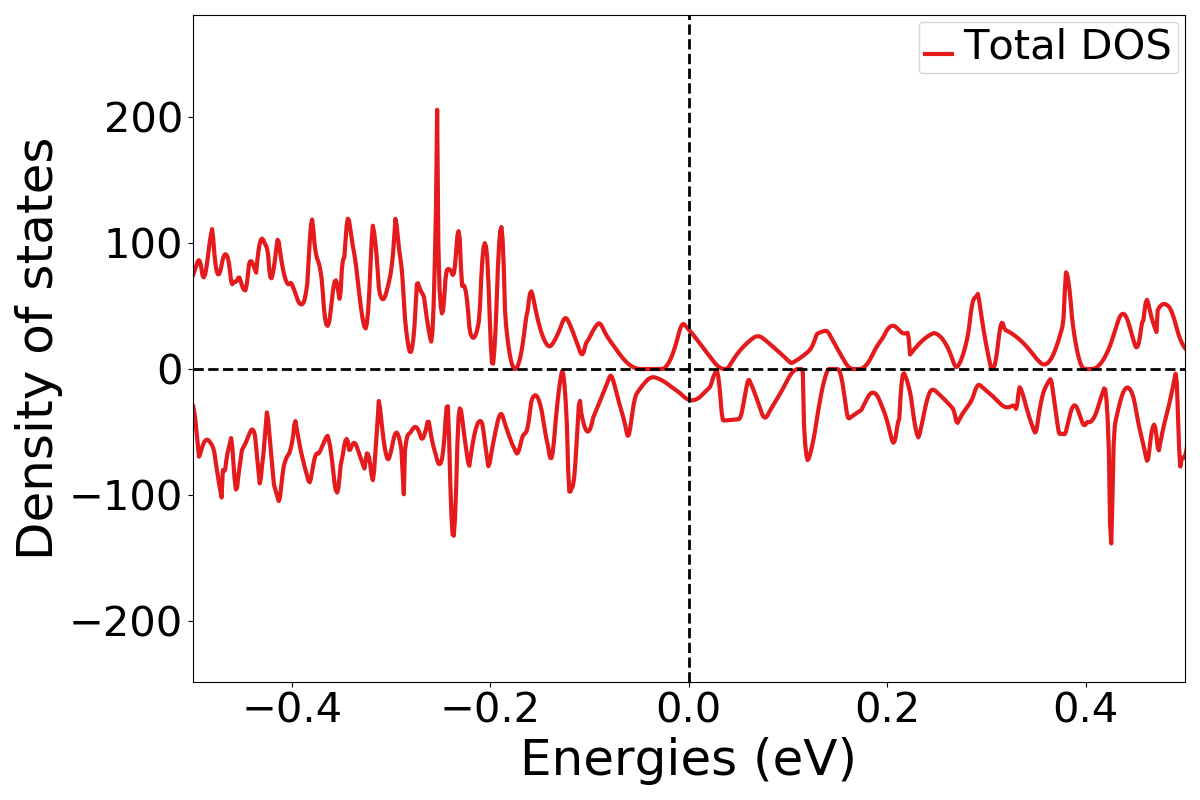
\includegraphics[width=.8\textwidth]{results/fesi2/192_E_DOS.png}
\caption{Density of states of SQS E 192 atom SQS.}
\end{figure}    
 
One could wonder if the very narrow band gap from the eigenvalues of $0.01$ eV is subject to numerical precision in the DOS. But on the grounds of the small value we calculated the DOS in this case by 20000 points over the energy range -12 eV to 12 eV which results in a resolution of about 8 points per 0.01 eV. In other words this should not be a factor of the DOS in figure 7.12. 
 
Drawing any conclusion on the band gaps is difficult seeing as we find very different results within all 3 sizes. The utmost stable SQSs suggests that the band gap converge towards a small or possible non-existent band gap with increasing SQS size. On the other hand we also find evidence of large band gaps in the larger cells in less stable configurations. This goes back to section 3.3 where we mentioned that one particular difficulty of the SQS method is the large number of possible atomic configurations of one composition. We should note that for the sake of comparison, we conducted the calculations of the larger SQSs with identical computational parameters as the 48-atom models, this could affect the accuracy of the larger structures.      

Looking at the pair distribution functions of the utmost stable SQS in each size (figure 7.13), we observe that short-range interactions is well represented and identical across all three models. The distinctions between preferences as discussed in section 7.2.4 is most likely a product of the uniqueness of the SQSs more so than the size. On the other hand the larger SQSs clearly provide a better description of large-range interactions, that is not nearly as present in the smaller supercell. But as seen from the minimal variation of the values in table 7.7 between the 3 models, in accordance with the fundamental philosophy of the SQS method that the functional properties are determined primarily from short-range interactions in the lattice. Thus, despite the fact that the larger SQSs offer improvement over the smaller SQSs, the gain is not justified by the cost. On the other hand, the SQS size looks to have more of an impact on the band gap of the material. But this could just as easily be a consequence of the sensitivity of the band gap to the particular atomic configuration as seen in table 7.8.

\begin{figure}[H]
\begin{subfigure}{\textwidth}
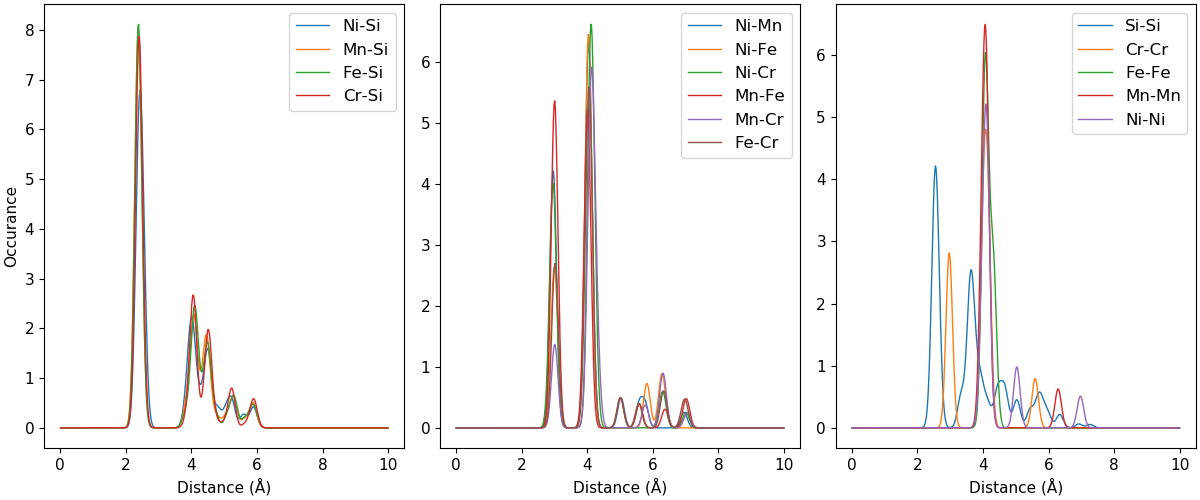
\includegraphics[width=\textwidth]{results/PDF48.png}
\end{subfigure}
\begin{subfigure}{\textwidth}
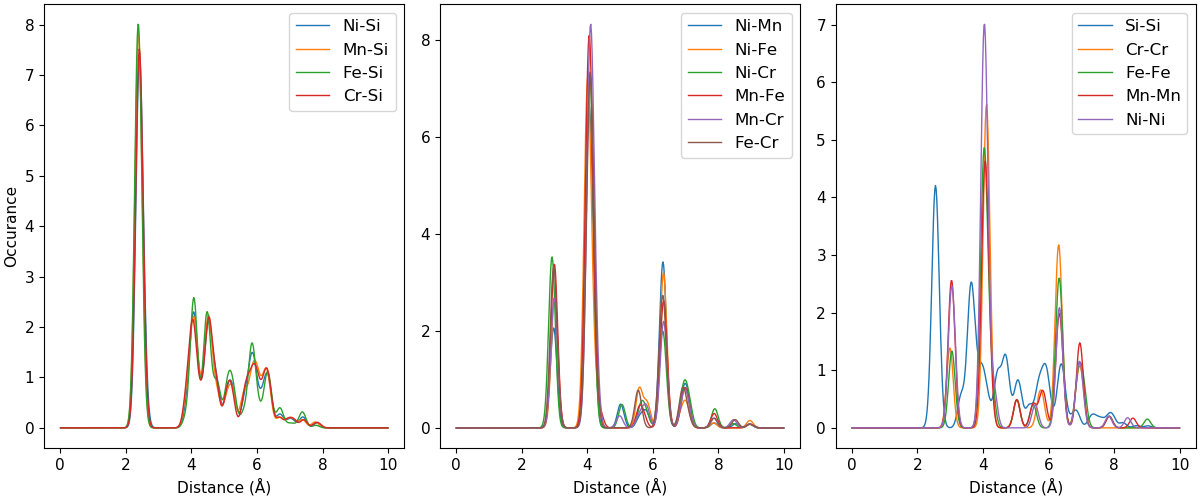
\includegraphics[width=\textwidth]{results/PDF96.png}
\end{subfigure}
\begin{subfigure}{\textwidth}
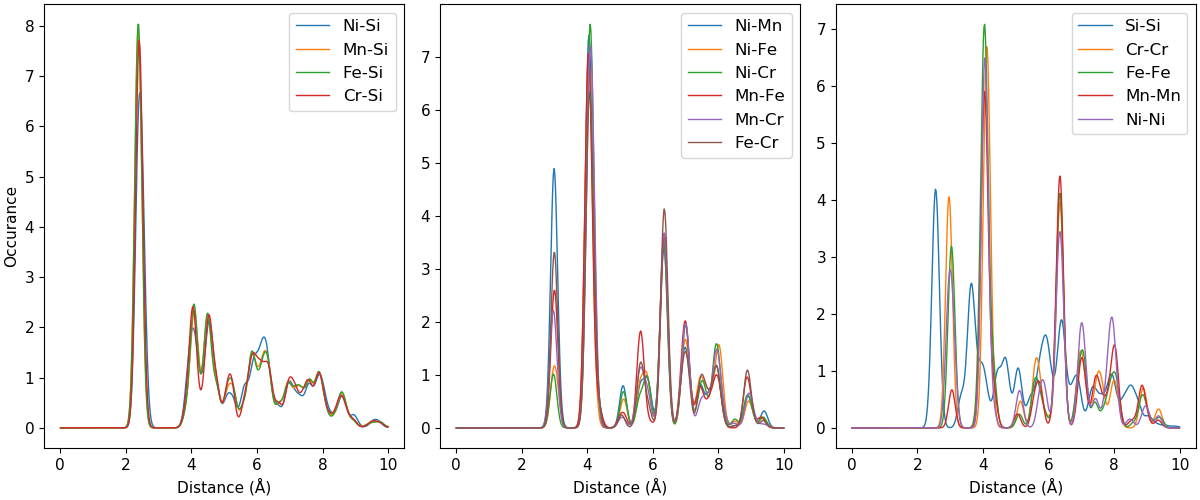
\includegraphics[width=\textwidth]{results/PDF192.png}
\end{subfigure}
\caption{Pair distribution functions of \ch{(CrFeMnNi)Si2} (top) 48-atom SQS, (middle) 96-atom SQS, (bottom) 192-atom SQS.}
\end{figure}
